\section{Frontend}\label{sec:poc:frontend}
Das Frontend ist über einen beliebigen Browser mit Websocket Unterstützung aufrufbar.
In \refFig{fig:frontend:poc:login} sieht man die Startseite des Frontends.
\begin{figure}[H]
  \centering
  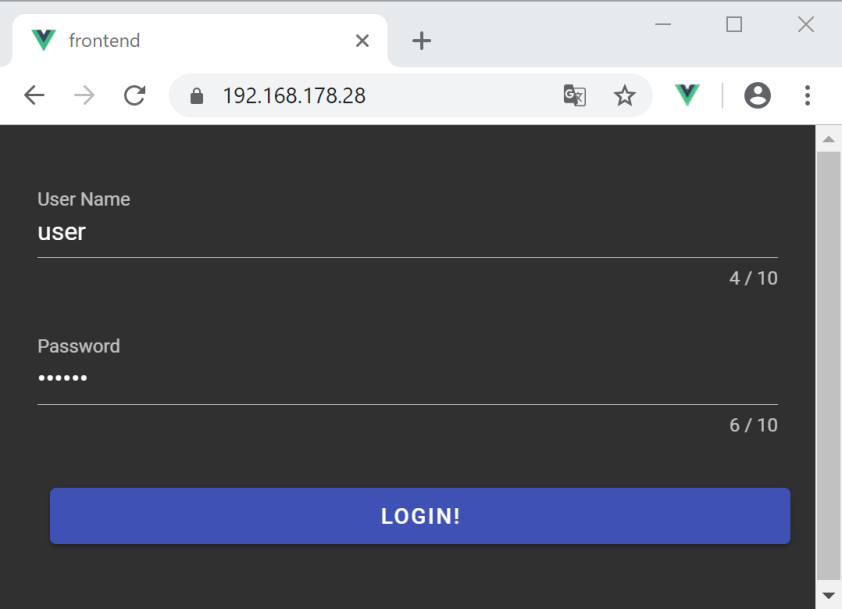
\includegraphics[width=0.8\textwidth]{content/hauptteil/umsetzungPoC/frontend/res/login.pdf}
  \caption{Screenshot der Login Seite im Browser}
  \label{fig:frontend:poc:login}
\end{figure}
Diese Seite ermöglicht die Authentifizierung ohne die eine weitere Interaktion mit dem Backend nicht möglich ist.
Hat man sich durch Eingabe, einem gültigen Passworts mit dem zugehöhrigen Benutzernamen, authentifiziert, 
so wird die erste Seite (\eigenName{ID = 1}) des \ac{scada} Systems angezeigt. In \refFig{fig:frontend:poc:page} ist diese Seite abgebildet.
\begin{figure}[ht]
  \centering
  
\includegraphics[width=0.8\textwidth]{content/hauptteil/umsetzungPoC/frontend/res/page.pdf}
  \caption{Screenshot einer Beispielseite}
  \label{fig:frontend:poc:page}
\end{figure}
Zur Veranschaulichung ist die Seite mit drei \ac{gui} Elementen gefüllt. 
Diese sind ein Textfelds (links), ein Button (mittig), sowie ein Label (rechts).
Das Textfeld hat die in \refFig{fig:frontend:poc:textFeld} dargestellten Darstellungsformen.
\begin{figure}[ht]
  \centering
  \hspace{0.05\textwidth}
  \begin{subfigure}[h]{0.24\textwidth}
    \centering
    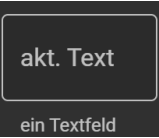
\includegraphics[width=\textwidth]{content/hauptteil/umsetzungPoC/frontend/res/TextfeldNoFokus.pdf}
    \caption{Textfeld \\ohne Fokus}
    \label{fig:frontend:poc:textFeld:noFocus}
  \end{subfigure}
  \hfill
  \begin{subfigure}[h]{0.24\textwidth}
    \centering
    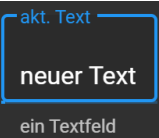
\includegraphics[width=\textwidth]{content/hauptteil/umsetzungPoC/frontend/res/TextfeldFokus.pdf}
    \caption{Textfeld \\editierbar}
    \label{fig:frontend:poc:textFeld:focus}
  \end{subfigure}
  \hfill
  \begin{subfigure}[h]{0.24\textwidth}
    \centering
    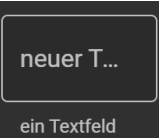
\includegraphics[width=\textwidth]{content/hauptteil/umsetzungPoC/frontend/res/TextfeldNeuerText.pdf}
    \caption{Textfeld \\nach Änderung}
    \label{fig:frontend:poc:textFeld:nachAenderung}
  \end{subfigure}
  \hspace{0.05\textwidth}
  \caption[Screenshot, Zustände eines Textfelds]{Screenshot eines Textfelds in drei verschiedenen Zuständen}
  \label{fig:frontend:poc:textFeld}
\end{figure}
Da die Architektur in Abschnitt \ref{subsec:archFrontend} es verbietet Ist- und Sollzustand in der selben Variablen zu speichern, sind diese Werte auch im Textfeld getrennt.
Wenn es nicht angeklickt wird, hat es nicht den Fokus und zeigt seinen aktuellen Wert an. 
Diese Darstellung ist in \refFig{fig:frontend:poc:textFeld:noFocus} zu sehen. unter dem Textfeld wird der Name des Felds angezeigt.
Wird das Textfeld angeklickt, ist es wie in \refFig{fig:frontend:poc:textFeld:focus} abgebildet, dargestellt. In diesem Zustand erlaubt es eine Eingabe durch den Nutzer.
Der aktuelle Wert wird dann im Rahmen angezeigt. 
Wenn das Textfeld abgewählt wird und damit den Fokus verliert, wird die Eingabe verworfen und es zeigt wieder den alten Wert an.
Wird die Eingabe mit \eigenName{Enter} bestätigt wird der neue Wert an das Backend gesendet. 
Das Textfeld zeigt diesen allerdings erst nach Bestätigung der Änderung durch das Backend an. 
In \refFig{fig:frontend:poc:textFeld:nachAenderung} sieht man den in \refFig{fig:frontend:poc:textFeld:focus} eingegeben neuen Wert \eigenNameNorm{neuer Text} in der gleichen Darstellungsform wie in \refFig{fig:frontend:poc:textFeld:noFocus} dargestellt.
Da der Text länger ist wie das Textfeld, wird dieser mit \eigenNameNorm{ \dots} abgekürzt.
\\Das \ac{gui} Element \eigenName{Button} hat die in \refFig{fig:frontend:poc:button} abgebildeten zwei Darstellungsformen.
\begin{figure}[ht]
  \centering
  \hspace{0.1\textwidth}
  \begin{subfigure}[h]{0.25\textwidth}
    \centering
    
\includegraphics[width=\textwidth]{content/hauptteil/umsetzungPoC/frontend/res/buttonTrue.pdf}
    \caption{\emph{DataNode} \\\eigenName{buttonState}=\emph{true}}
    \label{fig:frontend:poc:button:true}
  \end{subfigure}
  \hfill
  \begin{subfigure}[h]{0.25\textwidth}
    \centering
    
\includegraphics[width=\textwidth]{content/hauptteil/umsetzungPoC/frontend/res/buttonFalse.pdf}
    \caption{\emph{DataNode} \\\eigenName{buttonState}=\emph{false}}
    \label{fig:frontend:poc:button:false}
  \end{subfigure}
  \hspace{0.1\textwidth}
  \caption[Screenshot, Zustände eines Buttons]{Screenshot eines Buttons in zwei verschiedenen Zuständen}
  \label{fig:frontend:poc:button}
\end{figure}
Diese werden entsprechend der DataNode \emph{buttonState} ausgewählt. 
Durch das Klicken des Buttons wird der Wert der DataNode in ihren komplementären Wert geändert.
Der auf dem Button angezeigte Text, ist in einer \emph{ParamNode} gespeichert. Die Farbe des Buttons ist gemultiplext.
In einer \emph{ParamNode} ist ein \ac{json} Array gespeichert, das die einzelnen Farben enthält.
Diese können dann mit der \eigenName{colorSelector} \emph{DataNode} ausgewählt werden. 
\\Das dritte \ac{gui} Element auf der Beispielseite in \refFig{fig:frontend:poc:page} ist ein einfaches Label.
Der Text des Labels ist gemultiplext. \\Dieser Mechanismus ist analog zu der Farbe eines Buttons implementiert. 

\begin{figure}[ht]
  \centering
  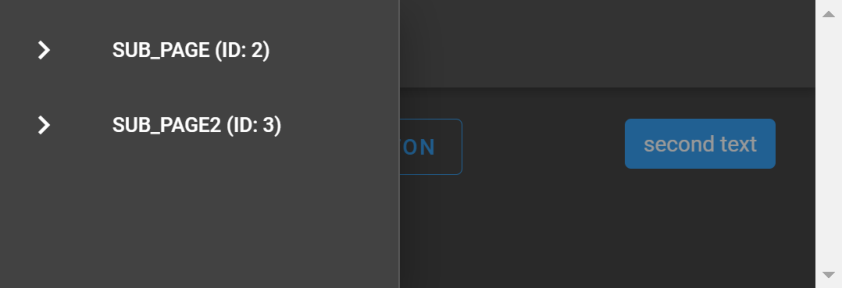
\includegraphics[width=0.8\textwidth]{content/hauptteil/umsetzungPoC/frontend/res/nav.pdf}
  \caption{Screenshot einer Beispielseite mit ausgeklappter Navigation}
  \label{fig:frontend:poc:page:nav}
\end{figure}
Um die Seite zu wechseln, kann man sich durch das Aufrufen der Navigationsleiste links, durch die Baumstruktur des \ac{scada} Systems navigieren.
Diese Leiste ist in \refFig{fig:frontend:poc:page:nav} dargestellt und wird durch den Button oben links in \refFig{fig:frontend:poc:page} eingeblendet.
Um die Navigation wieder auszublenden, muss in die Seite geklickt werden.